\Chapter{Megvalósítás}

\section{Fejlesztőkörnyezet előkészítése Windowson}

A feladat UNIX-alapú keretrendszer készítése, emiatt Windowson néhány előkészületre volt szükségem a fejlesztés elkezdése előtt. Először is, egy UNIX-alapú rendszerre van szükség WSL segítségével. Ehhez pedig, engedélyeznem kellett a WSL-t, majd telepíteni egy Linux disztribúciót \cite{wsl-install}. Ubuntura esett a választásom egyszerűsége és elterjedtsége miatt. A WSL-lel való fejlesztéshez pedig a Visual Studio Code-t (VSCode) ajánlja Microsoft és lett használva, emiatt pedig egy kiegészítőt is kellett telepíteni VSCode-hoz \cite{wsl+vscode}.

Grafikus alkalmazások fejlesztéséhez viszont szükség van az alábbi csomagokra is:
\begin{minted}{bash}
sudo apt install build-essential libx11-xcb-dev pkg-config
\end{minted}

Továbbá a grafikus felület látásához, szükség van egy X-szerver (például VcXsrv) telepítésére Windowson is, a fejlesztőfelület beállítására, hogy irányítsa át a megjelenítést a Windowson futó szervere, és végül a tűzfalon is állítani kellett \cite{vcxsrv-setup}.
Természetesen, egy új repository is létrehozásra került \textit{GitHub}-on.

\section{XCB használata}

Egy ablak megjelenítéséhez és az abba való rajzoláshoz UNIX alapú rendszeren X11 protokollt használva az XCB függvénykönyvtár és keretrendszer van használva. A keretrendszer használata bár egyszerűbb a többinél, még így is bonyolult, ezért leegyszerűsítő metódusokat hoztam létre. Továbbá a megértéséhez az XCB oldalán elérhető útmutatót használtam fel \cite{xcb-tutorial}. Az eredmény egy fehér ablak a képernyőn. A használt példa kód az útmutatóban megtalálható.

\subsection{Primitívek implementálása}

A primitívek és a Path primitívei implementálása egyszerű volt -- kivéve a görbéket -- ugyanis XCB is támogatta őket. A nem támogatottokat kihagytam idő nyerése érdekében. Példának alább egy téglalap körvonalát rajzoló segítő függvény kódja olvasható a \texttt{xcb-canvas} osztályból. Ez a kód XCB könyvtár segítségével az X-szervernek küldi el, hogy rajzolja ki a téglalap körvonalát az adott pozícióra és az adott dimenziókkal.

\begin{minted}{c}
void xcbcanvas_stroke_rectangle(
    xcbcanvas_t* canvas,
    int16_t x, int16_t y,
    uint16_t width, uint16_t height
)
{
  xcb_connection_t* c = canvas->connection;
  xcb_gcontext_t gc = canvas->gc;
  xcb_rectangle_t rectangle;
  rectangle.x = x;
  rectangle.y = y;
  rectangle.width = width;
  rectangle.height = height;
  xcb_poly_rectangle(c, canvas->window, gc, 1, &rectangle);
}
\end{minted}

Munkámat támogatta a Github Copilot technológiája is. A technológia segítségével gyorsabban tudtam implementálni a primitíveket és a Path primitíveit, hiszen a kódok nagyon hasonlóak.

Ezek után a függvénykönyvtár-felhasználó által használt kódot is implementáltam a \texttt{canvas} osztályban, a felső példát használva az alábbi módon. Ezek a metódusok már a teljes \texttt{canvas\_rendering\_context} globális adatait is kéri, és az argumentumok sorrendje a Canvas API sorrendjében vannak. Továbbá, az ebbe az osztályba kerülő metódusok részletesebb dokumentációt kapnak a header fájlokban.

\begin{minted}{c}
void canvas_stroke_rectangle(
    canvas_rendering_context_t* rendering_context,
    int16_t x, int16_t y,
    uint16_t width, uint16_t height
)
{
    xcbcanvas_stroke_rectangle(
        rendering_context->canvas, x, y, width, height);
}
\end{minted}

\subsection{Path implementálása}

A Path implementálására, egy dinamikusan növekedő tömböt implementáltam, amibe a Path primitíveit vagy egyéb utasításait tárolom. A dinamikus tömb 10 elemszámonként növekedik. Az alábbi példa a Path kezdését mutatja, illetve a kódpéldát dinamikus növekedésre.

\begin{minted}{c}
void canvas_begin_path(
    canvas_rendering_context_t* rendering_context
)
{
    rendering_context->path->sub_path_count = 0;
    rendering_context->path->sub_paths = malloc(sizeof(sub_path_t) * 10);
}

/* Továbbá minden egyéb Path utasítás elején: */
 if (rendering_context->path->sub_path_count % 10 == 9)
    {
        rendering_context->path->sub_paths = realloc(
            rendering_context->path->sub_paths,
            sizeof(sub_path_t) *
            (rendering_context->path->sub_path_count + 10));
    }
    int index = rendering_context->path->sub_path_count;
    sub_path_t* sub_path = &rendering_context->path->sub_paths[index];
\end{minted}

A Path befejezésekor a körvonal vagy a kitöltött választás alapján a megfelelő rajzoló függvényeket hívom meg. Bonyolultságot adott a Path-bezárás függvény implementációja, ugyanis menteni kell, hogy melyik pontra ugorjon vissza, és hogy egyáltalán ugorjon-e vissza arra a pontra. Az alábbi kód bemutatja a Path kirajzolás függvényét. Érdekes határeset, amikor csak egy primitív van a Path-ben ugyanis azt mindig csak egy mozgás utasításnak van véve.

% Kod felbontása és magyarázása

\begin{minted}{c}
void xcbcanvas_draw_path(xcbcanvas_t* canvas, path_t* path)
{
  if (path->sub_path_count == 0) {
    printf("Error: No sub-paths in path\n");
    return;
  }

  /*  Technically valid, but would do nothing
      since the first sub-path is treated as just a move to.
  */
  if (path->sub_path_count == 1) return;

  xcb_point_t current_position = path->sub_paths[0].point;
  xcb_point_t closing_point = path->sub_paths[0].point;
  /* Keep track of all the points
     that make up the shape that would need to be closed */
  xcb_point_t points[path->sub_path_count + 1];
  points[0] = current_position;
  uint16_t moves_since_close = 0;
  /* Render an outline path */
  if (!path->filled) {
    for (int i = 0; i < path->sub_path_count; i++) {
      switch (path->sub_paths[i].type) {
        case SUBPATH_TYPE_MOVE:
          /* Move pen to the given position */
          current_position = path->sub_paths[i].point;
          /* Add the point to the list of points
             that need to be closed */
          if (moves_since_close > 1)
            points[moves_since_close + 1] = closing_point;
          /* Reset moves since close counter */
          moves_since_close = 0;
          break;
        case SUBPATH_TYPE_LINE:
          /* Draw line between current position and the given one */
          xcbcanvas_line(canvas,
            current_position.x,
            current_position.y,
            path->sub_paths[i].point.x,
            path->sub_paths[i].point.y);
          /* Update currrent position */
          current_position = path->sub_paths[i].point;
          points[++moves_since_close] = current_position;
          break;
        case SUBPATH_TYPE_ARC:
          xcbcanvas_arc(canvas,
            path->sub_paths[i].point.x,
            path->sub_paths[i].point.y,
            path->sub_paths[i].arc.radius * 2,
            path->sub_paths[i].arc.radius * 2,
            path->sub_paths[i].arc.start_radius_or_cp2_x,
            path->sub_paths[i].arc.end_radius_or_cp2_y);
          break;
        case SUBPATH_TYPE_ARC_TO:
        case SUBPATH_TYPE_QUADRATIC_CURVE:
        case SUBPATH_TYPE_CUBIC_CURVE:
          printf("Error: Unsupported path sub-path type: %d\n",
            path->sub_paths[i].type);
          break;
        case SUBPATH_TYPE_CLOSE:
          /* Close the shape */
          if (moves_since_close > 1)
            points[moves_since_close + 1] = closing_point;
          xcbcanvas_line(canvas,
            current_position.x, current_position.y,
            closing_point.x, closing_point.y);
          current_position = path->sub_paths[0].point;
          break;
      }
    }
  }
  /* Render a filled path */
  else {
    /*  Same as above, but with the filled variants
    *   When closing a shape also need to make sure
    *   to correctly fill in the shape.
    */
    // [...]
  }
}
\end{minted}

\subsection{Szöveg implementálása}

Szöveg implementálásra az XCB két lehetőséget ad; egy elavult egyszerű módot, ahol csak néhány betűtípus és méret elérhető, illetve egy újabb komplikáltabb és flexibilisebbet. Az egyszerűbb verziót választottam, ugyanis annak az implementálása van benne az általam használt útmutatóban.

Az egyszerűbb verzióban először frissíteni (be kell tölteni) az X-szerverben tárolt adatot a használandó betűtípusról. Érdekesség, hogy a betűtípus azonosítója csak egy betűlánc, ami tárolja a nevét, méretét és egyéb tulajdonságait.

\begin{minted}{c}
void xcbcanvas_load_font(xcbcanvas_t* canvas, char* font_name)
{
  // First, create an id for the font
  xcb_font_t font = xcb_generate_id(canvas->connection);
  // Secondly, open the font
  xcb_void_cookie_t cookie =
    xcb_open_font_checked(
        canvas->connection, font, strlen(font_name), font_name);
  // Check for errors
  xcb_generic_error_t* error = xcb_request_check(
    canvas->connection, cookie);
  if (error)
  {
    fprintf(stderr, "Error opening font: %s\n", font_name);
    free(error);
    return;
  }
  // Then, assign font to our existing graphic context
  cookie = xcb_change_gc(
    canvas->connection, canvas->gc,
    XCB_GC_FONT, (uint32_t[]) { font });
  // Check for errors
  error = xcb_request_check(canvas->connection, cookie);
  if (error)
  {
    fprintf(stderr, "Error assigning font to graphic context\n");
    free(error);
    return;
  }
  // Close the font
  cookie = xcb_close_font_checked(canvas->connection, font);
  error = xcb_request_check(canvas->connection, cookie);
  if (error)
  {
    fprintf(stderr, "Error closing font\n");
    free(error);
    return;
  }
}
\end{minted}

Miután megadtuk az X-szervernek a betűtípust, felhasználhatjuk szöveg megjelenítéséhez az alábbi módon.

\begin{minted}{c}
void xcbcanvas_draw_text(
    xcbcanvas_t* canvas,
    int16_t x, int16_t y,
    const char* text)
{
  // Draw the text to the screen with the font that has been set
  xcb_void_cookie_t cookie_text = xcb_image_text_8_checked(
    canvas->connection, strlen(text),
    canvas->window, canvas->gc,
    x, y, text);
  xcb_generic_error_t* error =
    xcb_request_check(canvas->connection, cookie_text);
  if (error) {
    fprintf(stderr, "Error: Can't paste text: %d\n", error->error_code);
    free(error);
  }
}
\end{minted}

\subsection{További tervezett funkciók}

Primitívek, amelyek nem voltak az XCB-ben nem kerültek implementálásra. Például
\begin{itemize}
    \item a másodfokú és harmadfokú Bézier-görbe, ezekre léteznek már algoritmusok, amiket csak implementálni kell \cite{de-casteljau}, vagy
    \item \texttt{arcTo}, ami egy ív a kezdőponttól, két pont és egy sugár alapján.
\end{itemize}
Ez az ív úgy képzelhető el, hogy a kezdő- és első pont, illetve az első és második pont érintőegyenest alkot az ívnek. Emellett, a kezdőpontot és az ív tényleges kezdését egy vonallal kell összekötni. Ha pedig a sugarat növeljük, akkor az ív kerekebb lesz és távolabb kerül az első ponttól. Egy példa \texttt{arcTo}-ra látható \aref{fig:arcTo}. ábrán. Az \texttt{ArcTo}-ra nem tudom, hogy létezik-e hasonlóan megadott algoritmus, így lehetséges önállóan kell előállítani. Az ábrához használt kód alább olvasható.

\begin{minted}{javascript}
const canvas = document.getElementById('canvas');
const ctx = canvas.getContext('2d');
// Tangential lines
ctx.beginPath();
ctx.strokeStyle = 'gray';
ctx.moveTo(200, 20);
ctx.lineTo(200, 130);
ctx.lineTo(50, 20);
ctx.stroke();
// Arc
ctx.beginPath();
ctx.strokeStyle = 'black';
ctx.lineWidth = 5;
ctx.moveTo(200, 20);
ctx.arcTo(200,130, 50,20, 40);
ctx.stroke();
// Start point
ctx.beginPath();
ctx.fillStyle = 'blue';
ctx.arc(200, 20, 5, 0, 2 * Math.PI);
ctx.fill();
// Control points
ctx.beginPath();
ctx.fillStyle = 'red';
ctx.arc(200, 130, 5, 0, 2 * Math.PI); // Control point one
ctx.arc(50, 20, 5, 0, 2 * Math.PI);   // Control point two
ctx.fill();
\end{minted}

\begin{figure}
    \centering
    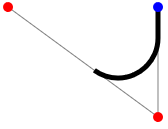
\includegraphics{images/arcTo.png}
    \caption{Példa \texttt{arcTo}-ra. A kék a kezdő pont, a piros pontok pedig a két másik végpont.}
    \label{fig:arcTo}
\end{figure}

Animáció implementálása többszálassá tenné programot, ugyanis utólag tudtam meg, hogy XCB csak akkor futtattja a rajzoló kódot, amikor egy ablak eddig takart része előtűnik (például megnyitás, tálcára minimalizálás visszavonása, takaró ablak elhúzása, aktív ablakká választás, ablak méret változtatása). Ez azt jelenti, hogy animáció implementáláshoz például egy külön szálon lenne szükség az időt tartanom, és egy eseményt küldeni a főszálnak, hogy frissüljön. A többszálas programok komplexitása miatt így nem implementáltam. A bemenet kezelésére nem tekintettem rá.

Továbbá, a Canvas API hatalmas, és nem mindenre tekintettem rá. Például átláthatóság, színkeverés, színátmenet, vagy akár kép betöltése mind olyan, amit nem sikerült lefedni, és nem is tudom, hogy XCB-ben hogyan lehetséges vagy az algoritmusokat nekem kell implementálni az előbb felsorolt dolgokhoz. Végül, az egységtesztelés is csak minimálisan lett implementálva.

\section{Egységtesztelés} \label{sec:cmocka-install}

Az XCB programok egységteszteléshez például a \textit{cmocka} függvénykönyvtár telepítésére és használatára van szükség (\url{https://cmocka.org}). A telepítéséhez letöltöttem a weboldaláról, kicsomagoltam, majd lefordítani a programot, végül a telepítőt rendszergazdaként futtattam. Ez a terminálban az alábbi módon tehető meg.

\begin{minted}{bash}
wget https://cmocka.org/files/1.1/cmocka-1.1.5.tar.xz
tar -xf cmocka-1.1.5.tar.xz
cd cmocka-1.1.5.tar.xz
mdkir build
cd build
cmake -DCMAKE_INSTALL_PREFIX=/usr -DCMAKE_BUILD_TYPE=Debug ..
make
sudo make install
\end{minted}

Ezután mockolással és tesztek készítésével, továbbá a \texttt{Makefile} módosításával lehetőség van automatikusan tesztelni a kódot minden fordításkor. A tesztek egy külön \texttt{tests} jegyzékben kaptak helyet. Alább a módosított \texttt{Makefile} olvasható.

\begin{minted}{Make}
tests: clean canvas.o xcb-canvas.o tests.o
	$(CC) $(STD) $(INCLUDE) -Wall -g tests/* \
	$(OUTPUT_FOLDER)/canvas.o $(OUTPUT_FOLDER)/xcb-canvas.o \
	$(OUTPUT_FOLDER)/tests.o \
	-o $(OUTPUT_FOLDER)/tests `$(PKG_CONF) xcb x11 cmocka` $(WRAP) && \
	./$(OUTPUT_FOLDER)/tests
tests.o:
	$(CC) $(STD) $(INCLUDE) -Wall -g -c src/tests.c \
	-o $(OUTPUT_FOLDER)/tests.o `$(PKG_CONF) cmocka` $(WRAP)
\end{minted}

Végül a teszteket meg is kellett írnom. Az egyik leggyakoribb teszt az a null mutatók elleni védelem. Egy ilyen tesztet mutat be az alábbi kód.

\begin{minted}{c}
void xcbcanvas_draw_path_test(void** state)
{
    xcbcanvas_draw_path(NULL, NULL);
    path_t* path;
    path = malloc(sizeof(path_t));
    path->sub_paths = NULL;
    xcbcanvas_draw_path(NULL, path);
    free(path);
}
\end{minted}

Mivel a kódom még nem volt védve null mutatók ellen, a sikertelen teszt üzenete várt:

\begin{verbatim}
[==========] Running 1 test(s).
[ RUN      ] xcbcanvas_draw_path_test
[  ERROR   ] --- Test failed with exception: Segmentation fault(11)
[  FAILED  ] xcbcanvas_draw_path_test
[==========] 1 test(s) run.
\end{verbatim}

Cmocka kiírja, hogy melyik teszt lett sikertelen és miért. Ez esetben, a null mutató \texttt{Segmentation fault}-ot okozott a programomban. A programomat javítottam az alábbi kód hozzáadásával.

\begin{minted}{c}
if (path == NULL) {
    printf("Error: Canvas path is NULL\n");
    return;
}
if (path->sub_paths == NULL) {
    printf("Error: Sub-paths is NULL\n");
    return;
}
\end{minted}

A kód hozzáadása után a teszt sikeressé is vált, amit a \textit{cmocka} az alábbi módon közölt velem. (Fontos megjegyezni, hogy a programomtól való hibaüzenetek várunk ebben az esetben.)

\begin{verbatim}
[==========] Running 1 test(s).
[ RUN      ] xcbcanvas_draw_path_test
Error: Canvas path is NULL
Error: Sub-paths is NULL
[       OK ] xcbcanvas_draw_path_test
[==========] 1 test(s) run.
\end{verbatim}

Hozzáadható lehetőség a repository-hoz, hogy mikor új kód kerül hozzáadásra, akkor azon automatikusan futtassa le ezeket a teszteket, és értesítse a fejlesztőket, ha valamelyik sikertelen.
